\documentclass[a4paper]{article}
\usepackage[italian]{babel}
\usepackage[italian]{isodate}  		% formato delle date in italiano
\usepackage{enumitem}				% gestione delle liste
\usepackage{pifont}					% pacchetto con elenchi carini
\usepackage[x11names]{xcolor}		% colori aggiuntivi
\usepackage{graphicx}
% Link ipertestuali per l'indice
%\usepackage{xcolor}
\usepackage[linkcolor=black, citecolor=blue, urlcolor=cyan]{hyperref}
\hypersetup{
	colorlinks=true
}

\newcommand{\dquotes}[1]{``#1''}

\begin{document}
	\title{Changelog}
	\date{\today}
	\maketitle
	
	\newpage
	
	\section*{Main Improvements}
	\begin{itemize}[label=\ding{51}]
		\item Modifica della \textsf{deepcopy}. C'erano dei problemi durante la ricreazione degli oggetti e i puntatori che venivano salvati. Tutto funzionava poiché anche se veniva effettuata la copia, gli oggetti originali non venivano utilizzati e quindi non avveniva nessuna collisione.
		
		\item Risolto il bug delle collisioni e dei drawer che si sovrascrivevano. Il bug era creato da questo indice:
		\begin{figure}[tph!]
			\centering
			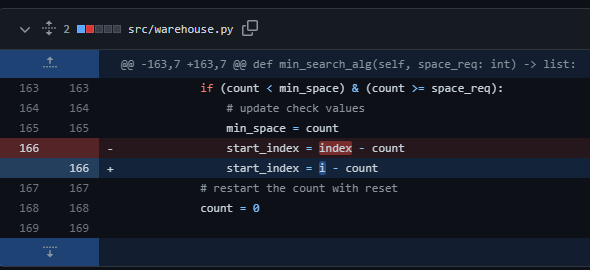
\includegraphics[width=\textwidth]{img/screenshot001}
			\label{fig:screenshot001}
		\end{figure}
		
		\item Rimossi tutti i print di debug.
		
		\item Modificata l'algoritmo per cercare la posizione, adesso ritorna solo valori che vengono effettivamente utilizzati. Risolto anche il bug dell'algoritmo di ricerca della posizione, poiché veniva selezionata sempre e solo una colonna, dato che nelle varie simulazioni non veniva mai riempita.
		
		\item Aggiunti alcuni parametri al file JSON:
		\begin{itemize}
			\item time $\rightarrow$ tempo di simulazione
			\item num\_actions $\rightarrow$ numero di azioni
			\item gen\_drawers $\rightarrow$ genera un numero di cassetti
			\item gen\_materials $\rightarrow$ genera un numero di materiali
			\item gen\_deposit $\rightarrow$ genera un cassetto anche nel deposito (IL CASSETTO NON È INCLUSO NELLA NUMERAZIONE DELLA GENERAZIONE DEI CASSETTI, cioè in gen\_drawers)
			\item gen\_buffer $\rightarrow$ genera un cassetto anche nel buffer (IL CASSETTO NON È INCLUSO NELLA NUMERAZIONE DELLA GENERAZIONE DEI CASSETTI, cioè in gen\_drawers)
		\end{itemize}
		
		\item Creazione del sito e refactoring delle cartelle.
		
		\item Aggiunto un dropdownmenu per scaricare il grafico in diversi formati.
	\end{itemize}
	
	\section*{Domande}
	\begin{itemize}
		\item
	\end{itemize}
\end{document}